% ============================================================================
% Neural Architecture Search for Function Approximation
% Duration: 45 minutes
% ============================================================================

\documentclass[aspectratio=169,11pt]{beamer}

% ---------- Theme and colors ----------
\usecolortheme{dove}
\setbeamertemplate{navigation symbols}{}
\setbeamertemplate{footline}{%
  \hfill\insertframenumber{}\hspace*{4pt}\vskip4pt}
\setbeamerfont{frametitle}{size=\huge}

% ---------- Packages ----------
\usepackage[utf8]{inputenc}
\usepackage[T1]{fontenc}
\usepackage{amsmath,amssymb,amsfonts}
\usepackage{bm}
\usepackage{graphicx}
\usepackage{tikz}
\usetikzlibrary{shapes,arrows.meta,positioning,calc,fit,backgrounds,patterns,decorations.pathreplacing}
\usepackage{pgfplots}
\pgfplotsset{compat=1.18}
\usepgfplotslibrary{fillbetween}
\usepackage{booktabs}
\usepackage{hyperref}
\usepackage{multicol}
\usepackage{xcolor}
\usepackage{algorithm}
\usepackage{algorithmic}

% ---------- Custom colors ----------
\definecolor{uzhblue}{rgb}{0,0,0.5}
\definecolor{uzhgreylight}{RGB}{236,238,241}
\definecolor{uzhgreydark}{RGB}{81,86,94}
\definecolor{harvardcrimson}{RGB}{153,0,0}
\definecolor{unil@blue}{RGB}{0,140,204}
\definecolor{unil@black}{RGB}{35,31,32}
\definecolor{darkgreen}{RGB}{0,100,0}
\definecolor{darkred}{RGB}{139,0,0}
\definecolor{softblue}{RGB}{70,130,180}
\definecolor{softorange}{RGB}{230,159,0}
\definecolor{softgreen}{RGB}{0,158,115}

% ---------- Set beamer colors ----------
\setbeamercolor{frametitle}{bg=uzhgreylight, fg=uzhblue}
\setbeamercolor{title}{fg=uzhblue}
\setbeamercolor{structure}{fg=uzhblue}
\setbeamercolor{block title}{bg=unil@blue, fg=white}
\setbeamercolor{block body}{bg=uzhgreylight}
\setbeamercolor{block title alerted}{bg=darkred,fg=white}
\setbeamercolor{block body alerted}{bg=red!5}
\setbeamercolor{block title example}{bg=darkgreen,fg=white}
\setbeamercolor{block body example}{bg=green!5}
\setbeamercolor{item}{fg=unil@black}
\setbeamercolor{normal text}{fg=unil@black}

% ---------- Emphasis and hyperlinks ----------
\newcommand{\emphc}[1]{\textcolor{harvardcrimson}{#1}}
\hypersetup{colorlinks,linkcolor=harvardcrimson,urlcolor=harvardcrimson}

% ---------- Math commands ----------
\newcommand{\x}{\bm{x}}
\newcommand{\w}{\bm{w}}
\newcommand{\bb}{\bm{b}}
\newcommand{\z}{\bm{z}}
\newcommand{\W}{\bm{W}}
\newcommand{\X}{\bm{X}}
\renewcommand{\a}{\bm{a}}
\newcommand{\R}{\mathbb{R}}
\newcommand{\E}[1]{\mathbb{E}\!\left[#1\right]}
\DeclareMathOperator*{\argmin}{arg\,min}
\DeclareMathOperator*{\argmax}{arg\,max}

% ---------- Title ----------
\title[NAS -- Padova 2026]%
{Deep Learning for Solving Dynamic Models}
\subtitle{Session 4a --- Neural architecture search: random search and Hyperband}
\author{Simon Scheidegger}
\institute[HEC Lausanne]{HEC, University of Lausanne}
\date{University of Padova\\September 23, 2026}

\begin{document}

% ============================================================================
% TITLE
% ============================================================================

% --- Slide 1: Title ---
{\setbeamercolor{background canvas}{bg=uzhgreylight}
\begin{frame}
\titlepage
\end{frame}
}

% --- Slide 2: Roadmap ---
\begin{frame}{Roadmap of This Lecture}
\begin{columns}[T]
\column{0.48\textwidth}
\textbf{I. Motivation}
\begin{itemize}
    \item Why architecture matters
    \item The hyperparameter space
    \item Limits of manual tuning
\end{itemize}

\vspace{0.4em}
\textbf{II. Search Methods}
\begin{itemize}
    \item Grid vs.\ random search
    \item Bayesian optimization
    \item Hyperband / successive halving
    \item Method comparison
\end{itemize}

\column{0.48\textwidth}
\textbf{III. Implementing the Search}
\begin{itemize}\itemsep0pt
    \item Defining a search space
    \item Random Search + SHA from scratch
    \item Tool landscape (footnote)
\end{itemize}

\vspace{0.4em}
\textbf{IV. Example \& Wrap-up}
\begin{itemize}\itemsep0pt
    \item Genz-function approximation
    \item Best practices
    \item Connection to DEQNs
\end{itemize}
\end{columns}

\vspace{0.2em}
\begin{center}
{\scriptsize Hands-on:
\texttt{02\_NAS\_Random\_Search\_10D.ipynb} (10-D random search)\\
\texttt{03\_NAS\_RandomSearch\_Hyperband.ipynb} (Random Search + SHA)}
\end{center}
\end{frame}

% --- Learning objectives ---
\begin{frame}{Learning objectives}
\textbf{By the end of this lecture you should be able to:}
\begin{itemize}
  \item Diagnose architecture sensitivity and quantify how network depth and width affect approximation error
  \item Compare grid search, random search, Bayesian optimization, and Hyperband on their computational cost and sample efficiency
  \item Implement random search and successive halving from scratch in plain Python
  \item Apply NAS to function approximation problems and choose appropriate search spaces for economic models
  \item Select production tools (KerasTuner, Optuna, Ray Tune) and apply best practices to scale architecture search efficiently
\end{itemize}
\end{frame}


% ============================================================================
% PART 1: MOTIVATION
% ============================================================================

% --- Slide 3: Why Architecture Matters ---
\begin{frame}{Why Architecture Matters}
\begin{columns}[T]
\column{0.52\textwidth}
\textbf{Same data, different architectures:}
\vspace{0.3cm}
\begin{itemize}
    \item 1 layer, 16 units $\;\Rightarrow\;$ MAE $= 0.08$
    \item 2 layers, 64 units $\;\Rightarrow\;$ MAE $= 0.01$
    \item 5 layers, 256 units $\;\Rightarrow\;$ MAE $= 0.003$
    \item 10 layers, 512 units $\;\Rightarrow\;$ MAE $= 0.02$ (overfit)
\end{itemize}
\vspace{0.3cm}
Architecture choice can matter \emphc{more than training duration}.

\vspace{0.25cm}
{\scriptsize\itshape Illustrative numbers from a depth/width sweep on the companion regression task; the from-scratch search in Notebook~03 reproduces the same ordering on a different testbed.}

\column{0.45\textwidth}
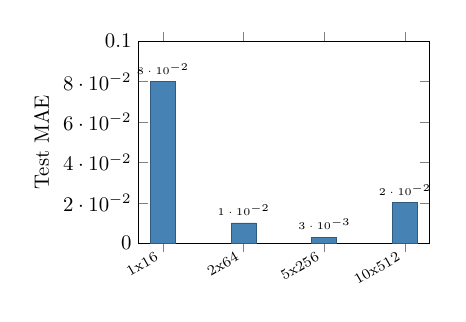
\begin{tikzpicture}[scale=0.75, transform shape]
    \begin{axis}[
        ybar,
        width=6.5cm, height=5cm,
        ylabel={Test MAE},
        symbolic x coords={1x16, 2x64, 5x256, 10x512},
        xtick=data,
        x tick label style={font=\scriptsize, rotate=30, anchor=east},
        ymin=0, ymax=0.1,
        bar width=12pt,
        nodes near coords,
        every node near coord/.append style={font=\tiny},
        nodes near coords align={vertical},
    ]
    \addplot[fill=softblue, draw=softblue!70!black] coordinates {
        (1x16, 0.08) (2x64, 0.01) (5x256, 0.003) (10x512, 0.02)
    };
    \end{axis}
\end{tikzpicture}
\end{columns}
\end{frame}

% --- Slide 3: The Hyperparameter Space ---
\begin{frame}{The Hyperparameter Space}
\begin{columns}[T]
\column{0.50\textwidth}
\textbf{Architectural hyperparameters:}
\begin{itemize}
    \item Number of hidden layers $L \in \{1, \ldots, 5\}$
    \item Units per layer $n_\ell \in \{32, 64, \ldots, 256\}$ (8 values)
    \item Activation: ReLU, tanh, swish
\end{itemize}

\vspace{0.3cm}
\textbf{Training hyperparameters:}
\begin{itemize}
    \item Learning rate $\eta$ log-uniform on $[10^{-4}, 10^{-2}]$ (20-point grid)
    \item Batch size $B \in \{16, 32, 64, 128\}$
    \item Epochs, regularization, \ldots
\end{itemize}

\column{0.47\textwidth}
\begin{block}{Combinatorial explosion}
Even this modest search space:
\[
    |\mathcal{H}| = 5 \times 8 \times 3 \times 20 \times 4 = \emphc{9{,}600}
\]
\vspace{-0.2cm}
\begin{itemize}
    \item Each trial: minutes to hours
    \item Full grid: \emphc{infeasible}
\end{itemize}
\end{block}
\end{columns}
\end{frame}

% --- Slide 4: Manual Tuning ---
\begin{frame}{Manual Tuning}
\begin{columns}[T]
\column{0.55\textwidth}
\textbf{The ``grad-student descent'' approach:}
\begin{enumerate}
    \item Pick an architecture (intuition / paper)
    \item Train, evaluate, adjust one thing
    \item Repeat until deadline
\end{enumerate}

\vspace{0.3cm}
\textbf{Problems:}
\begin{itemize}
    \item \emphc{Doesn't scale} beyond a few hyperparameters
    \item \emphc{Human bias}: we try what we already know
    \item \emphc{Not reproducible}: results depend on the researcher
    \item Misses interactions between hyperparameters
\end{itemize}

\column{0.42\textwidth}
\vspace{0.5cm}
\begin{block}{Key insight}
We need \textbf{automated, systematic} methods to search the hyperparameter space efficiently.
\end{block}
\end{columns}
\end{frame}

% ============================================================================
% PART 2: AUTOMATED SEARCH STRATEGIES
% ============================================================================

% --- Slide 5: Section Divider ---
{\setbeamercolor{background canvas}{bg=uzhblue}
\setbeamercolor{normal text}{fg=white}
\usebeamercolor[fg]{normal text}
\begin{frame}[plain,c]
\begin{center}
{\Huge\bfseries Automated Search Strategies}
\end{center}
\end{frame}
}

% --- Slide 6: Grid Search ---
\begin{frame}{Grid Search}
\begin{columns}[T]
\column{0.52\textwidth}
\textbf{Idea:} Enumerate all combinations on a regular grid.

\vspace{0.3cm}
\begin{block}{Algorithm}
\begin{enumerate}
    \item Define discrete set for each HP
    \item Evaluate \emph{every} combination
    \item Return the best
\end{enumerate}
\end{block}

\vspace{0.2cm}
\textbf{Cost:} $\mathcal{O}(k^d)$ --- exponential in dimension $d$.

\vspace{0.2cm}
\textbf{Pros:} Simple, embarrassingly parallel.

\textbf{Cons:} Wastes budget on \emphc{unimportant} dimensions.

\column{0.45\textwidth}
\begin{center}
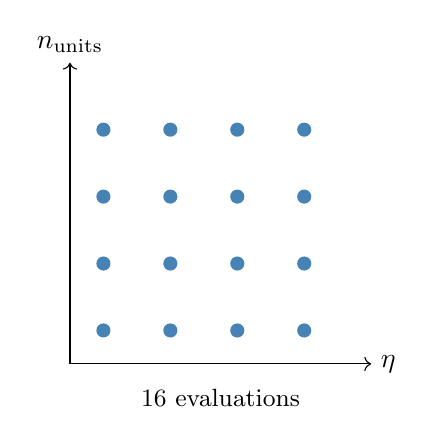
\begin{tikzpicture}[scale=0.85]
    \draw[->] (0,0) -- (4.5,0) node[right] {$\eta$};
    \draw[->] (0,0) -- (0,4.5) node[above] {$n_\text{units}$};
    % Grid points
    \foreach \xi in {0.5,1.5,2.5,3.5} {
        \foreach \yi in {0.5,1.5,2.5,3.5} {
            \fill[softblue] (\xi,\yi) circle (3pt);
        }
    }
    \node[font=\small] at (2.25,-0.5) {16 evaluations};
\end{tikzpicture}
\end{center}
\end{columns}
\end{frame}

% --- Slide 7: Random Search ---
\begin{frame}{Random Search}
\begin{columns}[T]
\column{0.52\textwidth}
\textbf{Idea:} Sample configurations uniformly at random.

\vspace{0.2cm}
\begin{block}{Key result (Bergstra \& Bengio, 2012)}
When only a \emph{few} dimensions matter, random search finds good configurations with \emphc{fewer trials} than grid search.
\end{block}

\vspace{0.2cm}
\textbf{Why?} Random points explore each dimension \emph{independently} --- more unique values per HP.

\vspace{0.2cm}
\textbf{Cost:} $\mathcal{O}(n)$ --- linear in budget $n$.

\column{0.45\textwidth}
\begin{center}
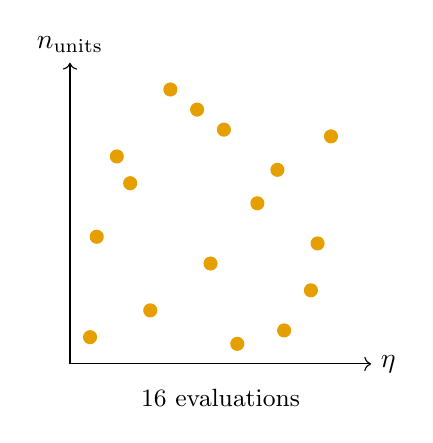
\begin{tikzpicture}[scale=0.85]
    \draw[->] (0,0) -- (4.5,0) node[right] {$\eta$};
    \draw[->] (0,0) -- (0,4.5) node[above] {$n_\text{units}$};
    % Random points (fixed seed for reproducibility)
    \fill[softorange] (0.7,3.1) circle (3pt);
    \fill[softorange] (1.2,0.8) circle (3pt);
    \fill[softorange] (2.8,2.4) circle (3pt);
    \fill[softorange] (3.6,1.1) circle (3pt);
    \fill[softorange] (0.4,1.9) circle (3pt);
    \fill[softorange] (1.9,3.8) circle (3pt);
    \fill[softorange] (3.2,0.5) circle (3pt);
    \fill[softorange] (2.1,1.5) circle (3pt);
    \fill[softorange] (0.9,2.7) circle (3pt);
    \fill[softorange] (3.9,3.4) circle (3pt);
    \fill[softorange] (1.5,4.1) circle (3pt);
    \fill[softorange] (2.5,0.3) circle (3pt);
    \fill[softorange] (3.1,2.9) circle (3pt);
    \fill[softorange] (0.3,0.4) circle (3pt);
    \fill[softorange] (2.3,3.5) circle (3pt);
    \fill[softorange] (3.7,1.8) circle (3pt);
    \node[font=\small] at (2.25,-0.5) {16 evaluations};
\end{tikzpicture}
\end{center}
\end{columns}
\end{frame}

% --- Slide 8: Grid vs Random Visual ---
\begin{frame}{Grid vs.\ Random --- Why Random Wins}
\begin{center}
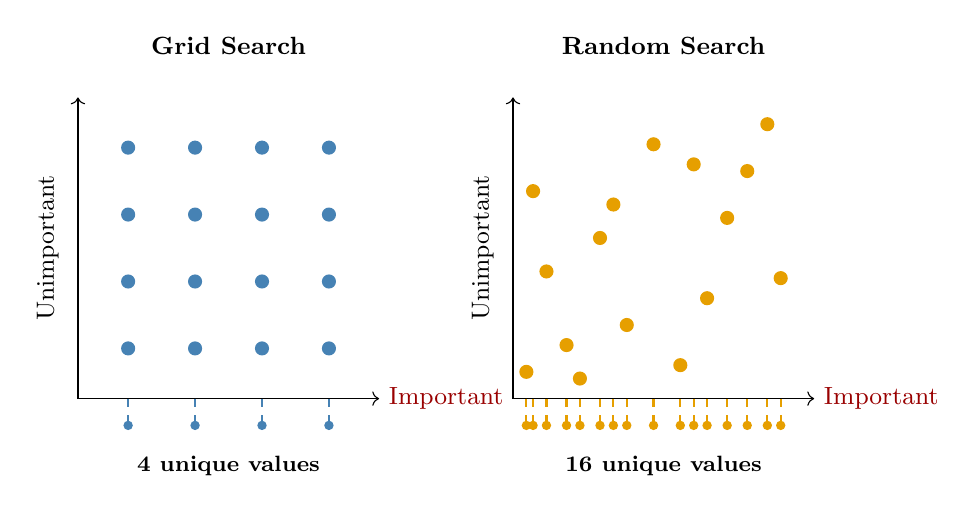
\begin{tikzpicture}[scale=0.85]
    % --- Left panel: Grid ---
    \begin{scope}[shift={(0,0)}]
        \draw[->] (0,0) -- (4.5,0) node[right,font=\small] {\emphc{Important}};
        \draw[->] (0,0) -- (0,4.5);
        \node[font=\small, rotate=90] at (-0.45,2.25) {Unimportant};
        \foreach \xi in {0.75,1.75,2.75,3.75} {
            \foreach \yi in {0.75,1.75,2.75,3.75} {
                \fill[softblue] (\xi,\yi) circle (3pt);
            }
        }
        % Project onto x-axis
        \foreach \xi in {0.75,1.75,2.75,3.75} {
            \draw[softblue, thick, dashed] (\xi,0) -- (\xi,-0.4);
            \fill[softblue] (\xi,-0.4) circle (2pt);
        }
        \node[font=\footnotesize] at (2.25,-1.0) {\textbf{4 unique values}};
        \node[font=\small, above] at (2.25,5.0) {\textbf{Grid Search}};
    \end{scope}

    % --- Right panel: Random ---
    \begin{scope}[shift={(6.5,0)}]
        \draw[->] (0,0) -- (4.5,0) node[right,font=\small] {\emphc{Important}};
        \draw[->] (0,0) -- (0,4.5);
        \node[font=\small, rotate=90] at (-0.45,2.25) {Unimportant};
        % Random points
        \fill[softorange] (0.3,3.1) circle (3pt);
        \fill[softorange] (0.8,0.8) circle (3pt);
        \fill[softorange] (1.3,2.4) circle (3pt);
        \fill[softorange] (1.7,1.1) circle (3pt);
        \fill[softorange] (0.5,1.9) circle (3pt);
        \fill[softorange] (2.1,3.8) circle (3pt);
        \fill[softorange] (2.5,0.5) circle (3pt);
        \fill[softorange] (2.9,1.5) circle (3pt);
        \fill[softorange] (3.2,2.7) circle (3pt);
        \fill[softorange] (3.5,3.4) circle (3pt);
        \fill[softorange] (3.8,4.1) circle (3pt);
        \fill[softorange] (1.0,0.3) circle (3pt);
        \fill[softorange] (1.5,2.9) circle (3pt);
        \fill[softorange] (0.2,0.4) circle (3pt);
        \fill[softorange] (2.7,3.5) circle (3pt);
        \fill[softorange] (4.0,1.8) circle (3pt);
        % Project onto x-axis
        \foreach \xi in {0.2,0.3,0.5,0.8,1.0,1.3,1.5,1.7,2.1,2.5,2.7,2.9,3.2,3.5,3.8,4.0} {
            \draw[softorange, thick, dashed] (\xi,0) -- (\xi,-0.4);
            \fill[softorange] (\xi,-0.4) circle (2pt);
        }
        \node[font=\footnotesize] at (2.25,-1.0) {\textbf{16 unique values}};
        \node[font=\small, above] at (2.25,5.0) {\textbf{Random Search}};
    \end{scope}
\end{tikzpicture}
\end{center}

\vspace{0.1cm}
{\small When one dimension matters, the grid wastes most evaluations on the
unimportant axis; random search samples the important axis more densely.}
\end{frame}

% --- Slide 9: Bayesian Optimization ---
\begin{frame}{Bayesian Optimization}
\begin{columns}[T]
\column{0.55\textwidth}
\textbf{Idea:} Build a \emph{surrogate model} of $f(\text{HP}) \to \text{loss}$ and use it to choose the next trial \emph{intelligently}.

\vspace{0.3cm}
\begin{enumerate}
    \item Fit a Gaussian process (GP) to observed trials
    \item Compute an \emphc{acquisition function} (e.g., Expected Improvement)
    \item Evaluate the HP with highest acquisition value
    \item Update the GP and repeat
\end{enumerate}

\vspace{0.3cm}
\textbf{Key advantage:} \emphc{Sample-efficient} --- exploits structure in the response surface.

\column{0.42\textwidth}
\begin{block}{Expected Improvement}
\vspace{-0.2cm}
\[
    \text{EI}(\x) = \E{\max(f^* - f(\x), 0)}
\]
\vspace{-0.2cm}
\begin{itemize}
    \item $f^*$: best observed value
    \item Balances \emph{exploration} (high uncertainty) and \emph{exploitation} (low predicted loss)
\end{itemize}
\end{block}
\end{columns}
\end{frame}

% --- Slide 10: Bayesian Optimization Visual ---
\begin{frame}{Bayesian Optimization --- Visual}
\begin{center}
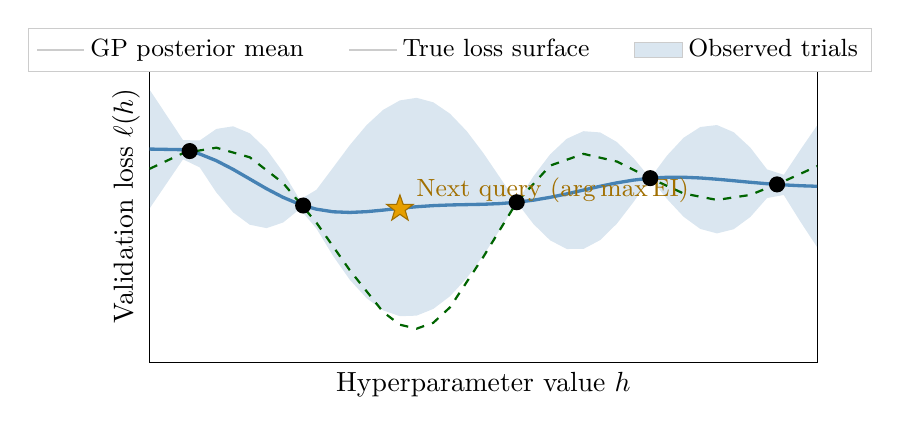
\begin{tikzpicture}[scale=0.9]
    \begin{axis}[
        width=11cm, height=6cm,
        xlabel={Hyperparameter value $h$},
        ylabel={Validation loss $\ell(h)$},
        xmin=0, xmax=10, ymin=-1.3, ymax=1.0,
        xtick=\empty, ytick=\empty,
        legend style={at={(0.5,1.03)}, anchor=south, legend columns=-1,
                      font=\small, /tikz/every even column/.append style={column sep=0.5cm},
                      draw=gray!40, fill=white},
        clip=false,
    ]
    % Uncertainty band (+-2 sigma) from a genuine RBF-GP fit
    \addplot[name path=upper, draw=none] coordinates {
      (0.000,+0.7045) (0.500,+0.3347) (0.750,+0.3315) (1.000,+0.4166) (1.250,+0.4359) (1.500,+0.3846) (1.750,+0.2677) (2.000,+0.0984) (2.250,-0.1036) (2.500,-0.0299) (2.750,+0.1338) (3.000,+0.2983) (3.250,+0.4445) (3.500,+0.5573) (3.750,+0.6262) (4.000,+0.6451) (4.250,+0.6120) (4.500,+0.5286) (4.750,+0.4008) (5.000,+0.2390) (5.250,+0.0584) (5.500,-0.1221) (5.750,+0.0683) (6.000,+0.2297) (6.250,+0.3446) (6.500,+0.4000) (6.750,+0.3908) (7.000,+0.3206) (7.250,+0.2019) (7.500,+0.0546) (7.750,+0.2200) (8.000,+0.3518) (8.250,+0.4307) (8.500,+0.4452) (8.750,+0.3927) (9.000,+0.2795) (9.250,+0.1195) (9.500,+0.0797) (9.750,+0.2634) (10.000,+0.4417)
    };
    \addplot[name path=lower, draw=none] coordinates {
      (0.000,-0.1673) (0.500,+0.1932) (0.750,+0.1339) (1.000,-0.0503) (1.250,-0.1964) (1.500,-0.2871) (1.750,-0.3122) (2.000,-0.2709) (2.250,-0.1715) (2.500,-0.3161) (2.750,-0.5179) (3.000,-0.6921) (3.250,-0.8270) (3.500,-0.9166) (3.750,-0.9591) (4.000,-0.9549) (4.250,-0.9055) (4.500,-0.8126) (4.750,-0.6796) (5.000,-0.5125) (5.250,-0.3218) (5.500,-0.1221) (5.750,-0.2819) (6.000,-0.4016) (6.250,-0.4655) (6.500,-0.4650) (6.750,-0.4000) (7.000,-0.2794) (7.250,-0.1203) (7.500,+0.0546) (7.750,-0.0971) (8.000,-0.2286) (8.250,-0.3181) (8.500,-0.3508) (8.750,-0.3205) (9.000,-0.2302) (9.250,-0.0912) (9.500,-0.0686) (9.750,-0.2648) (10.000,-0.4512)
    };
    \addplot[fill=softblue, fill opacity=0.20] fill between[of=upper and lower];

    % GP posterior mean (interpolates all 5 observations)
    \addplot[softblue, very thick] coordinates {
      (0.000,+0.2686) (0.500,+0.2640) (0.600,+0.2538) (0.750,+0.2327) (1.000,+0.1832) (1.250,+0.1197) (1.500,+0.0488) (1.750,-0.0223) (2.000,-0.0862) (2.250,-0.1375) (2.300,-0.1459) (2.500,-0.1730) (2.750,-0.1921) (3.000,-0.1969) (3.250,-0.1912) (3.500,-0.1796) (3.750,-0.1664) (4.000,-0.1549) (4.250,-0.1467) (4.500,-0.1420) (4.750,-0.1394) (5.000,-0.1368) (5.250,-0.1317) (5.500,-0.1221) (5.750,-0.1068) (6.000,-0.0859) (6.250,-0.0605) (6.500,-0.0325) (6.750,-0.0046) (7.000,+0.0206) (7.250,+0.0408) (7.500,+0.0546) (7.750,+0.0614) (8.000,+0.0616) (8.250,+0.0563) (8.500,+0.0472) (8.750,+0.0361) (9.000,+0.0246) (9.250,+0.0142) (9.400,+0.0087) (9.500,+0.0056) (9.750,-0.0007) (10.000,-0.0047)
    };
    \addlegendentry{GP posterior mean}

    % True function (hidden dip near h=4.2)
    \addplot[darkgreen, thick, dashed] coordinates {
      (0.000,+0.1238) (0.500,+0.2382) (1.000,+0.2786) (1.500,+0.2082) (2.000,+0.0189) (2.500,-0.2730) (3.000,-0.6221) (3.500,-0.9293) (3.750,-1.0217) (4.000,-1.0505) (4.250,-1.0071) (4.500,-0.8939) (5.000,-0.5230) (5.500,-0.1221) (6.000,+0.1471) (6.500,+0.2334) (7.000,+0.1771) (7.500,+0.0546) (8.000,-0.0577) (8.500,-0.1050) (9.000,-0.0681) (9.500,+0.0315) (10.000,+0.1427)
    };
    \addlegendentry{True loss surface}

    % Observed points
    \addplot[only marks, mark=*, mark size=3pt, black]
      coordinates {(0.60,+0.254) (2.30,-0.146) (5.50,-0.122) (7.50,+0.055) (9.40,+0.009)};
    \addlegendentry{Observed trials}

    % Next query: EI peak at h = 3.75 (picked from the same GP)
    \node[star, star points=5, star point ratio=2.5, fill=softorange, draw=softorange!70!black,
          minimum size=10pt, inner sep=0pt] at (axis cs:3.75,-0.17) {};
    \node[font=\small, softorange!70!black, above right] at (axis cs:3.85,-0.20) {Next query ($\arg\max\mathrm{EI}$)};
    \end{axis}
\end{tikzpicture}
\end{center}

\vspace{-0.2em}
\small The GP posterior mean \emph{interpolates} the five observations and is \emph{wide} in unexplored gaps.  The Expected-Improvement acquisition function peaks at $h \approx 3.75$, trading off the high posterior variance there against the moderately low predicted mean.
\end{frame}

% --- Slide 11: Hyperband ---
\begin{frame}{Hyperband}
\footnotesize
\begin{columns}[T]
\column{0.55\textwidth}
\textbf{Idea:} Start many configurations cheaply; \emphc{stop the worst early} and give more resources to promising ones.

\vspace{0.05cm}
\begin{block}{Successive Halving (SHA, $\eta=3$)}
\begin{enumerate}\itemsep0pt
    \item Start $n$ random configs with budget $b$
    \item Train each for $b$ epochs, evaluate
    \item \emphc{Keep the top $1/\eta$} of configs (discard the rest)
    \item Multiply the budget by $\eta$, repeat
\end{enumerate}
\end{block}

\textbf{Hyperband} = SHA with several brackets (different $n/b$ trade-offs), each bracket itself being a stage cascade like $9 \to 3 \to 1$ above.  The usual default is $\eta=3$.

\textbf{Resource use:} many cheap trials; full budgets only for survivors.

\column{0.42\textwidth}
\textbf{Key insight:}
\begin{itemize}\itemsep0pt
    \item Bad configs identifiable \emph{early}
    \item No need for 200 epochs to know $\eta\!=\!10$ diverges
    \item Exploits \emphc{correlation} between early and late performance
\end{itemize}

{\scriptsize Li et al.\ (2018): large speedups when early and late performance are correlated.}
\end{columns}
\end{frame}

% --- Slide 12: Hyperband Visual ---
\begin{frame}{Hyperband --- Successive Halving}
\begin{center}
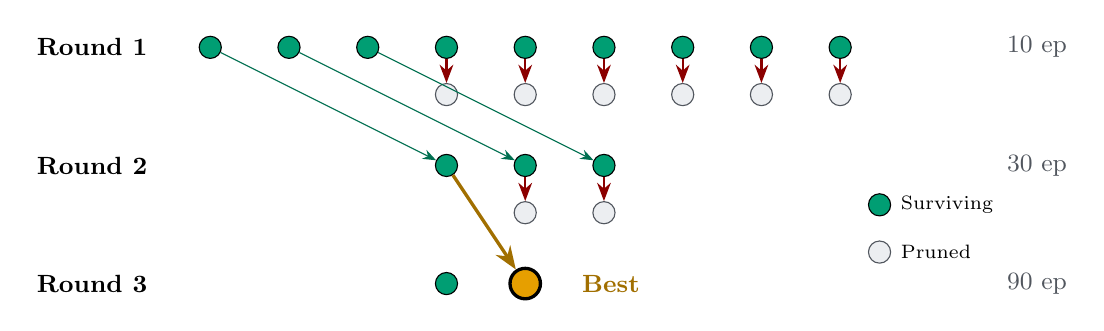
\begin{tikzpicture}[
    trialnode/.style={circle, draw, minimum size=8pt, inner sep=0pt},
    alive/.style={trialnode, fill=softgreen},
    dead/.style={trialnode, fill=uzhgreylight, draw=uzhgreydark},
    >=Stealth,
]
    % Round labels (factor eta = 3 cascade: 9 -> 3 -> 1)
    \node[font=\small\bfseries] at (-1.5, 0) {Round 1};
    \node[font=\small\bfseries] at (-1.5,-1.5) {Round 2};
    \node[font=\small\bfseries] at (-1.5,-3.0) {Round 3};

    % Epoch labels (each round triples the budget)
    \node[font=\small, uzhgreydark] at (10.5, 0) {10 ep};
    \node[font=\small, uzhgreydark] at (10.5,-1.5) {30 ep};
    \node[font=\small, uzhgreydark] at (10.5,-3.0) {90 ep};

    % Round 1: 9 trials
    \foreach \i in {0,...,8} {
        \node[alive] (r1-\i) at (\i*1.0, 0) {};
    }

    % Round 2: 3 survive (top 1/3)
    \foreach \i in {0,...,2} {
        \node[alive] (r2-\i) at (\i*1.0 + 3.0, -1.5) {};
    }
    \foreach \i in {3,...,8} {
        \node[dead] (r1d-\i) at (\i*1.0, -0.6) {};
        \draw[->, darkred, thick] (r1-\i) -- (r1d-\i);
    }
    % Arrows from survivors
    \draw[->, softgreen!70!black] (r1-0) -- (r2-0);
    \draw[->, softgreen!70!black] (r1-1) -- (r2-1);
    \draw[->, softgreen!70!black] (r1-2) -- (r2-2);

    % Round 3: 1 survives (top 1/3 of 3)
    \foreach \i in {0} {
        \node[alive] (r3-\i) at (\i*1.2 + 3.0, -3.0) {};
    }
    % Round 3 (winner from 3): keep top 1/3 = 1
    \node[alive, fill=softorange, minimum size=11pt, line width=1.2pt] (r3-0) at (4.0, -3.0) {};
    \foreach \i in {1,2} {
        \node[dead] (r2d-\i) at (\i*1.0 + 3.0, -2.1) {};
        \draw[->, darkred, thick] (r2-\i) -- (r2d-\i);
    }
    \draw[->, softorange!70!black, line width=1.2pt] (r2-0) -- (r3-0);
    \node[font=\small\bfseries, softorange!70!black, right] at (4.6,-3.0) {Best};

    % Legend
    \node[alive, label={right:\scriptsize Surviving}] at (8.5, -2.0) {};
    \node[dead, label={right:\scriptsize Pruned}] at (8.5, -2.6) {};
\end{tikzpicture}
\end{center}

\vspace{0.1cm}
$9 \to 3 \to 1$ (factor $\eta=3$): total cost $= 9 \times 10 + 3 \times 30 + 1 \times 90
= \emphc{270}$ epoch-equivalents (vs.\ $9 \times 90 = 810$ for full training).

\vspace{0.05cm}
{\scriptsize \textbf{Bracket vs.\ schedule.}  This $9 \to 3 \to 1$ cascade is one SHA bracket.  Hyperband itself runs several brackets in parallel, each with a different starting $(n, b)$ trade-off, hedging across the unknown correlation between early- and late-training performance.}
\end{frame}

% --- Slide 13: Method Comparison ---
\begin{frame}{Method Comparison}
\begin{center}
\renewcommand{\arraystretch}{1.3}
{\small
\begin{tabular}{@{}lcccc@{}}
\toprule
\textbf{Property} & \textbf{Grid} & \textbf{Random} & \textbf{Bayesian} & \textbf{Hyperband} \\
\midrule
Computational cost & $\mathcal{O}(k^d)$ & $\mathcal{O}(n)$ & $\mathcal{O}(n)$ & $\mathcal{O}(n \log n)$ \\
Sample efficiency & Low & Medium & \emphc{High} & High \\
Parallelisable & Fully & Fully & Limited & Partially \\
Handles interactions & No & Partially & \emphc{Yes} & No \\
Early stopping & No & No & No & \emphc{Yes} \\
Implementation & Trivial & Trivial & Moderate & Moderate \\
\bottomrule
\end{tabular}
}
\end{center}

\vspace{0.4cm}
\textbf{Practical advice:}
\begin{itemize}
    \item \textbf{Quick exploration:} Random search (strong baseline)
    \item \textbf{Limited budget:} Bayesian optimization (sample-efficient)
    \item \textbf{Large search space:} Hyperband (aggressive early stopping)
\end{itemize}
\end{frame}

% ============================================================================
% PART 3: IMPLEMENTING THE SEARCH (FROM SCRATCH)
% ============================================================================

% --- Slide 14: Section Divider ---
{\setbeamercolor{background canvas}{bg=uzhblue}
\setbeamercolor{normal text}{fg=white}
\usebeamercolor[fg]{normal text}
\begin{frame}[plain,c]
\begin{center}
{\Huge\bfseries Implementing the Search}\\[0.3cm]
{\large\itshape Random Search and Successive Halving, from scratch}
\end{center}
\end{frame}
}

% --- Slide 15: Defining a Search Space (plain Python) ---
\begin{frame}[fragile]{Defining a Search Space}
\begin{block}{A plain dict --- no library required}
{\scriptsize
\begin{verbatim}
SPACE = {
    "layers":     [1, 2, 3, 4, 5],
    "units":      [32, 64, 96, 128, 160, 192, 224, 256],
    "activation": ["relu", "tanh", "swish"],
    "lr":         ("log_uniform", 1e-4, 1e-2),
}
def sample_config(rng):
    return {
        "layers":     int(rng.choice(SPACE["layers"])),
        "units":      int(rng.choice(SPACE["units"])),
        "activation": str(rng.choice(SPACE["activation"])),
        "lr":         float(10 ** rng.uniform(-4, -2)),
    }
\end{verbatim}
}
\end{block}
{\scriptsize No \texttt{hp.Int} / \texttt{hp.Float} abstraction --- the search space is a dict, the sampler is one function.}
\end{frame}

% --- Slide 16: Random Search from scratch ---
\begin{frame}[fragile]{Random Search from Scratch}
\begin{block}{30 trials, single function}
{\scriptsize
\begin{verbatim}
def random_search(n_trials=30, epochs=50, seed=0):
    rng = np.random.default_rng(seed)
    records = []
    for t in range(n_trials):
        cfg = sample_config(rng)
        model = build_model(cfg)
        h = model.fit(X_tr, y_tr, epochs=epochs,
                      validation_data=(X_val, y_val), verbose=0)
        records.append((cfg, min(h.history["val_loss"])))
    return min(records, key=lambda r: r[1])
\end{verbatim}
}
\end{block}
{\scriptsize Independent uniform draws; $\mathcal{O}(N)$ cost, embarrassingly parallel (Bergstra \& Bengio, 2012).}
\end{frame}

% --- Slide 17: Successive Halving from scratch ---
\begin{frame}[fragile]{Successive Halving from Scratch}
\begin{block}{$n_0=27$, $\eta=3$, three rounds}
{\scriptsize
\begin{verbatim}
def successive_halving(n0=27, eta=3, r0=8, seed=0):
    rng = np.random.default_rng(seed)
    survivors = [(sample_config(rng), None) for _ in range(n0)]
    r = r0
    while len(survivors) > 1:
        scored = [(cfg, train_for(cfg, epochs=r)) for cfg, _ in survivors]
        scored.sort(key=lambda s: s[1])           # ascending val loss
        keep   = max(1, len(scored) // eta)
        survivors = scored[:keep]
        r *= eta                                  # 8 -> 24 -> 72 epochs
    return survivors[0]
\end{verbatim}
}
\end{block}
{\scriptsize Notebook schedule: 27 candidates @ 8 ep $\to$ 9 @ 24 ep $\to$ 3 @ 72 ep $\to$ 1 winner.  This is $648$ config-epochs, versus $1500$ for $30$ random-search trials at $50$ epochs each: about $2.3\times$ less compute while testing a comparable number of architectures.}
\end{frame}

% --- Slide 18: Tool landscape (footnote) ---
\begin{frame}{Production Tooling (footnote)}
We just wrote both algorithms in $\sim$25 lines of Python.  Real projects rarely hand-roll the loop; established libraries wrap (and parallelise) the same algorithms behind a uniform API:

\vspace{0.3cm}
\begin{center}
\renewcommand{\arraystretch}{1.15}
{\small
\begin{tabular}{@{}lll@{}}
\toprule
\textbf{Library} & \textbf{Algorithms} & \textbf{Notes} \\
\midrule
\href{https://keras.io/keras_tuner/}{KerasTuner}   & Random, Bayesian, Hyperband      & Tight Keras integration \\
\href{https://optuna.org/}{Optuna}                 & TPE, CMA-ES, Hyperband, NSGA-II  & Framework-agnostic; popular default \\
\href{https://docs.ray.io/en/latest/tune/}{Ray Tune} & All of the above + ASHA, PBT     & Distributed by design \\
\href{http://hyperopt.github.io/hyperopt/}{Hyperopt} & TPE, Random                      & The original TPE reference \\
\href{https://ax.dev/}{Ax / BoTorch}               & Bayesian (multi-objective, MOO)  & Meta; PyTorch-native GPs \\
\href{https://nni.readthedocs.io/}{NNI}            & Random, Bayesian, evolutionary, NAS & Microsoft; full graph-NAS support \\
\bottomrule
\end{tabular}}
\end{center}

\vspace{0.15cm}
{\scriptsize\textbf{Why teach algorithms, not wrappers.}  APIs change; the search loops (Random, SHA/Hyperband, GP+EI, TPE) persist.}
\end{frame}

% ============================================================================
% PART 4: EXAMPLE --- GENZ FUNCTION APPROXIMATION
% ============================================================================

% --- Slide 19: Section Divider ---
{\setbeamercolor{background canvas}{bg=uzhblue}
\setbeamercolor{normal text}{fg=white}
\usebeamercolor[fg]{normal text}
\begin{frame}[plain,c]
\begin{center}
{\Huge\bfseries Example: Genz Function}\\[0.3cm]
{\Large\bfseries Approximation}
\end{center}
\end{frame}
}

% --- Slide 20: Setup ---
\begin{frame}{Experiment Setup}
\begin{columns}[T]
\column{0.52\textwidth}
\textbf{Target function:} Genz Gaussian on $[0,1]^2$
\[
    f(\x) = \exp\!\Bigl(-\sum_{i=1}^{d} c_i^2 (x_i - w_i)^2\Bigr)
\]

\vspace{0.2cm}
\textbf{Data:}
\begin{itemize}
    \item $d = 2$, uniform random samples
    \item $n_\text{train} = 1{,}000$, $n_\text{test} = 2{,}000$
    \item Loss: MSE, metric: test MAE
\end{itemize}

\column{0.45\textwidth}
\textbf{Search space:}
\begin{itemize}
    \item Layers: $1$--$5$
    \item Units/layer: $32$--$256$ (step 32)
    \item Activation: ReLU, tanh, swish
    \item LR: $10^{-4}$--$10^{-2}$ (log scale)
\end{itemize}

\vspace{0.3cm}
\textbf{Baseline:} $3 \times 64$ ReLU MLP, $\eta = 10^{-3}$

\vspace{0.2cm}
\textbf{Budget:} 30 trials per method
\end{columns}
\end{frame}

% --- Slide 21: Search Results ---
\begin{frame}{Search Results (Random Search vs.\ SHA on a 2-D Genz Gaussian)}
\begin{center}
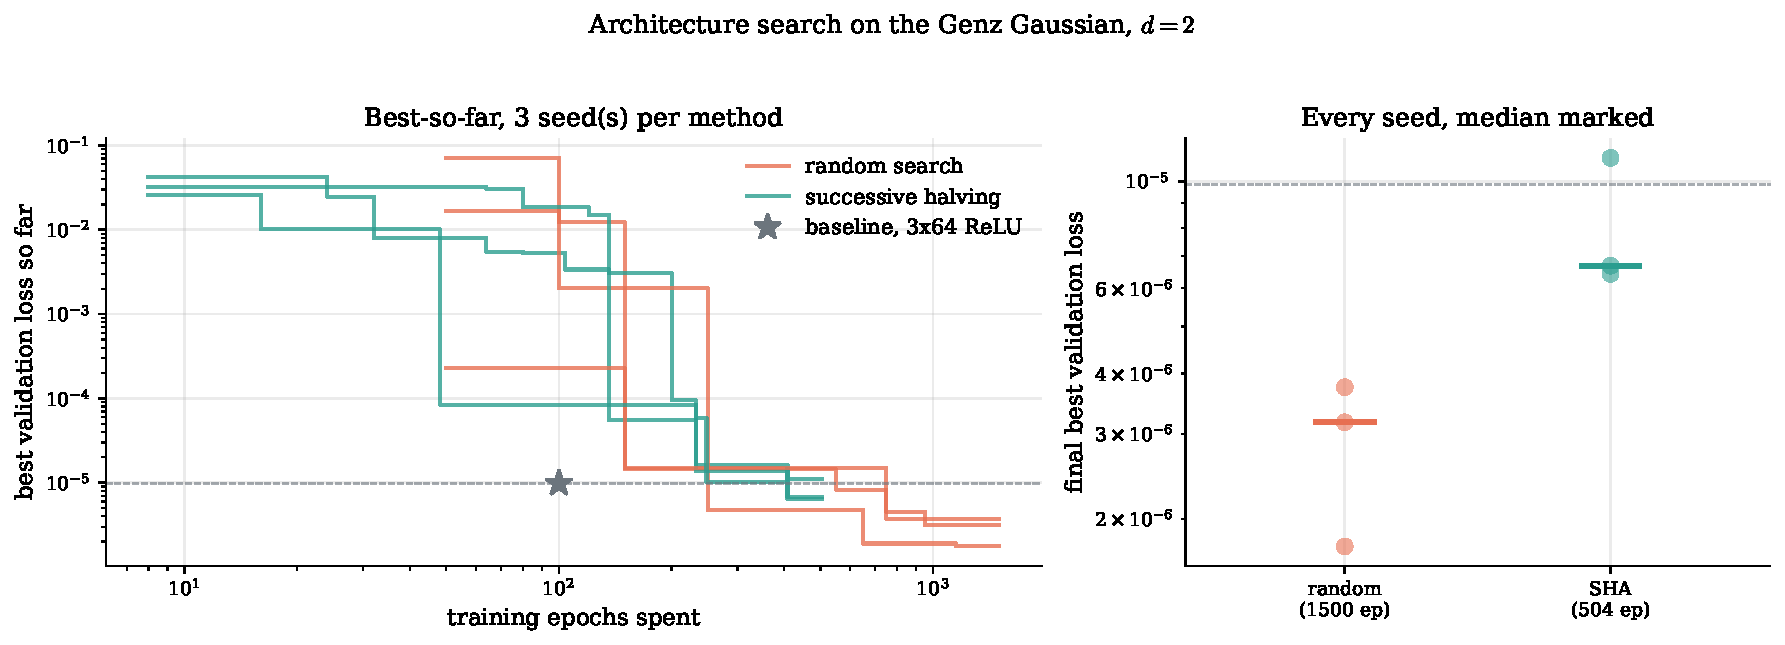
\includegraphics[width=0.92\linewidth]{figures/nas_search_results.pdf}
\end{center}

\vspace{-0.4em}
{\scriptsize Generated by \texttt{03\_NAS\_RandomSearch\_Hyperband.ipynb}.  Random Search uses $30$ full trials; SHA uses $27$ initial candidates with $\eta=3$.  Both reach MAE of order $10^{-3}$ from a baseline near $4\cdot10^{-3}$; SHA uses about $2.3\times$ less config-epoch budget in this seeded run.}
\end{frame}

% --- Slide 22: Visualization ---
\begin{frame}{Best Model vs.\ Ground Truth}
\begin{center}
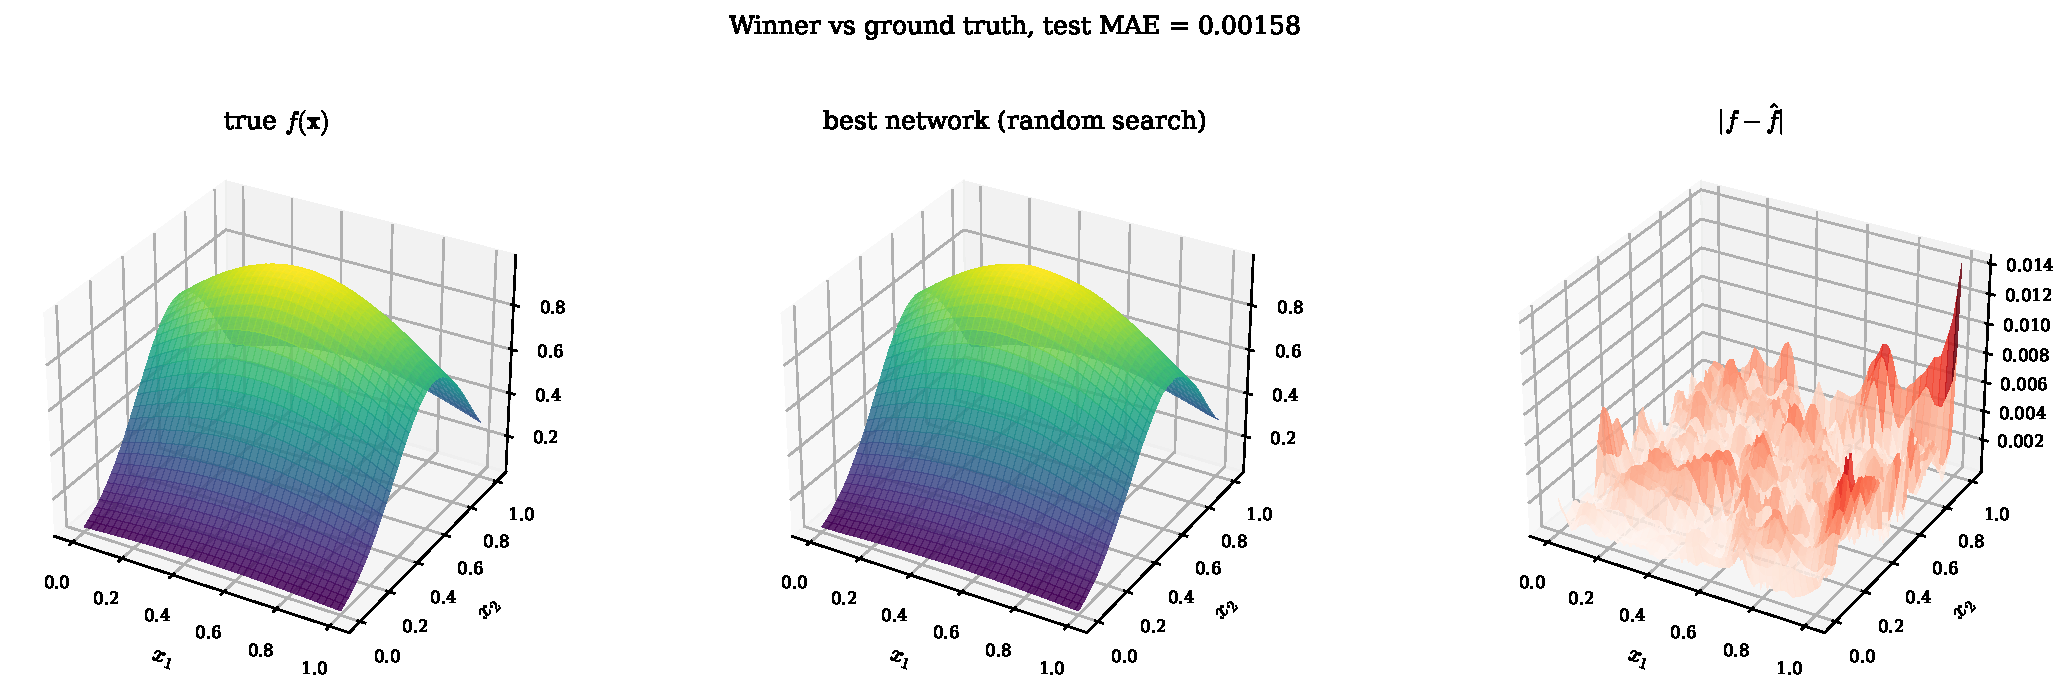
\includegraphics[width=0.92\linewidth]{figures/nas_best_surface.pdf}
\end{center}

\vspace{-0.2em}
{\footnotesize Generated by \texttt{03\_NAS\_RandomSearch\_Hyperband.ipynb}.  Left to right: the true Genz target, the best NAS-found NN approximation, and the absolute error map on $[0,1]^2$.  No placeholder shapes; this is the actual notebook output.  The companion \texttt{02\_NAS\_Random\_Search\_10D.ipynb} offers a 10-D testbed (search loop in plain Python, model in TF/Keras).}
\end{frame}

% --- Slide 23: Best Practices ---
\begin{frame}{Best Practices for NAS}
\begin{columns}[T]
\column{0.50\textwidth}
\textbf{Search space design:}
\begin{itemize}
    \item Start small, expand if needed
    \item Use \emphc{log-scale} for learning rate
    \item Constrain to reasonable ranges
    \item Include the current best as a point
\end{itemize}

\vspace{0.3cm}
\textbf{Budget allocation:}
\begin{itemize}
    \item Diminishing returns after $\sim$30 trials
    \item Hyperband: set \texttt{factor=3} (default)
    \item Use early stopping callbacks
\end{itemize}

\column{0.47\textwidth}
\textbf{Common pitfalls:}
\begin{itemize}
    \item Search space too large $\Rightarrow$ wasted budget
    \item Overfitting to validation set $\Rightarrow$ use holdout test
    \item Ignoring training stability $\Rightarrow$ check learning curves
\end{itemize}

\vspace{0.3cm}
\begin{alertblock}{Rule of thumb}
If manual tuning took $N$ trials, automated search with $3N$ trials will likely find something better.
\end{alertblock}
\end{columns}
\end{frame}

% --- Slide 24: Connection to Economics ---
\begin{frame}{Connection to Economics}
\textbf{Where NAS matters in computational economics:}

\vspace{0.3cm}
\begin{enumerate}
    \item \textbf{Surrogate models:} Replace expensive simulations (e.g., climate IAMs) with NNs --- architecture determines approximation quality.

    \vspace{0.2cm}
    \item \textbf{DSGE policy functions:} Deep equilibrium nets (Lecture 03) use NNs to approximate policy/value functions. \emphc{Architecture search over the policy network} can improve convergence.

    \vspace{0.2cm}
    \item \textbf{High-dimensional problems:} As $d$ grows (many state variables), the architecture must scale. NAS automates this adaptation.

    \vspace{0.2cm}
    \item \textbf{Reproducibility:} Automated search documents \emph{which} architectures were tried, making results more transparent than ``we chose 3 layers with 64 units.''
\end{enumerate}
\end{frame}

% --- Slide 25: Summary + References ---
\begin{frame}{Summary}
\begin{columns}[T]
\column{0.55\textwidth}
\textbf{Key takeaways:}
\begin{enumerate}
    \item Architecture choice \emphc{strongly} affects NN performance
    \item Random search is a strong baseline --- always try it first
    \item Bayesian optimization is most sample-efficient
    \item Hyperband / SHA offers the best speed/quality trade-off
    \item Production: KerasTuner, Optuna, Ray Tune, Ax all wrap these
\end{enumerate}

\column{0.42\textwidth}
\textbf{References:}
{\scriptsize
\begin{itemize}\itemsep0pt
    \item \emphc{Elsken, Metzen \& Hutter (2019)} --- \emph{NAS: A Survey}, JMLR 20(55).
    \item Bergstra \& Bengio (2012). \emph{Random search.} JMLR 13.
    \item Li et al.\ (2018). \emph{Hyperband.} JMLR 18(185).
    \item Garnett (2023). \emph{Bayesian optimization.} CUP.
    \item Snoek et al.\ (2012). \emph{Practical Bayesian optimization.} NeurIPS.
\end{itemize}
}
\end{columns}

\end{frame}

\end{document}
